\section{Literature Review}
\label{sec:review}
%

\subsection{Introduction}
\subsubsection{Overview on smart devices}

Advances in communication and control technologies have led to the rise of internet controlled devices that change the way we live and work. An increase in computer processing power and energy-efficient sensors has made smart devices economically feasible. Smart devices comprise a physical component, a “smart” component and a connectivity component that allows the functions of the device to exist outside the physical component and connect with your smartphone. Smart components, such as sensors, microprocessors and software distinguish the conventional devices from smart devices as they allow a person to switch on the product just once and allow it to perform its functions without any more user input. The connectivity components such as antennae enable wireless connections with the product, allowing a user to control a device remotely. The control of the temperature of a room can now be accomplished using an internet-connected thermostat, allowing the user to monitor and control the heat settings of a room remotely on a smartphone while some systems are programmed to automatically lower or increase the temperature in a room \cite{noauthor_3_nodate}. The future of tomorrow is in smart homes such as the one shown in figure \ref{fig:smarthome}

\begin{figure}[ht]
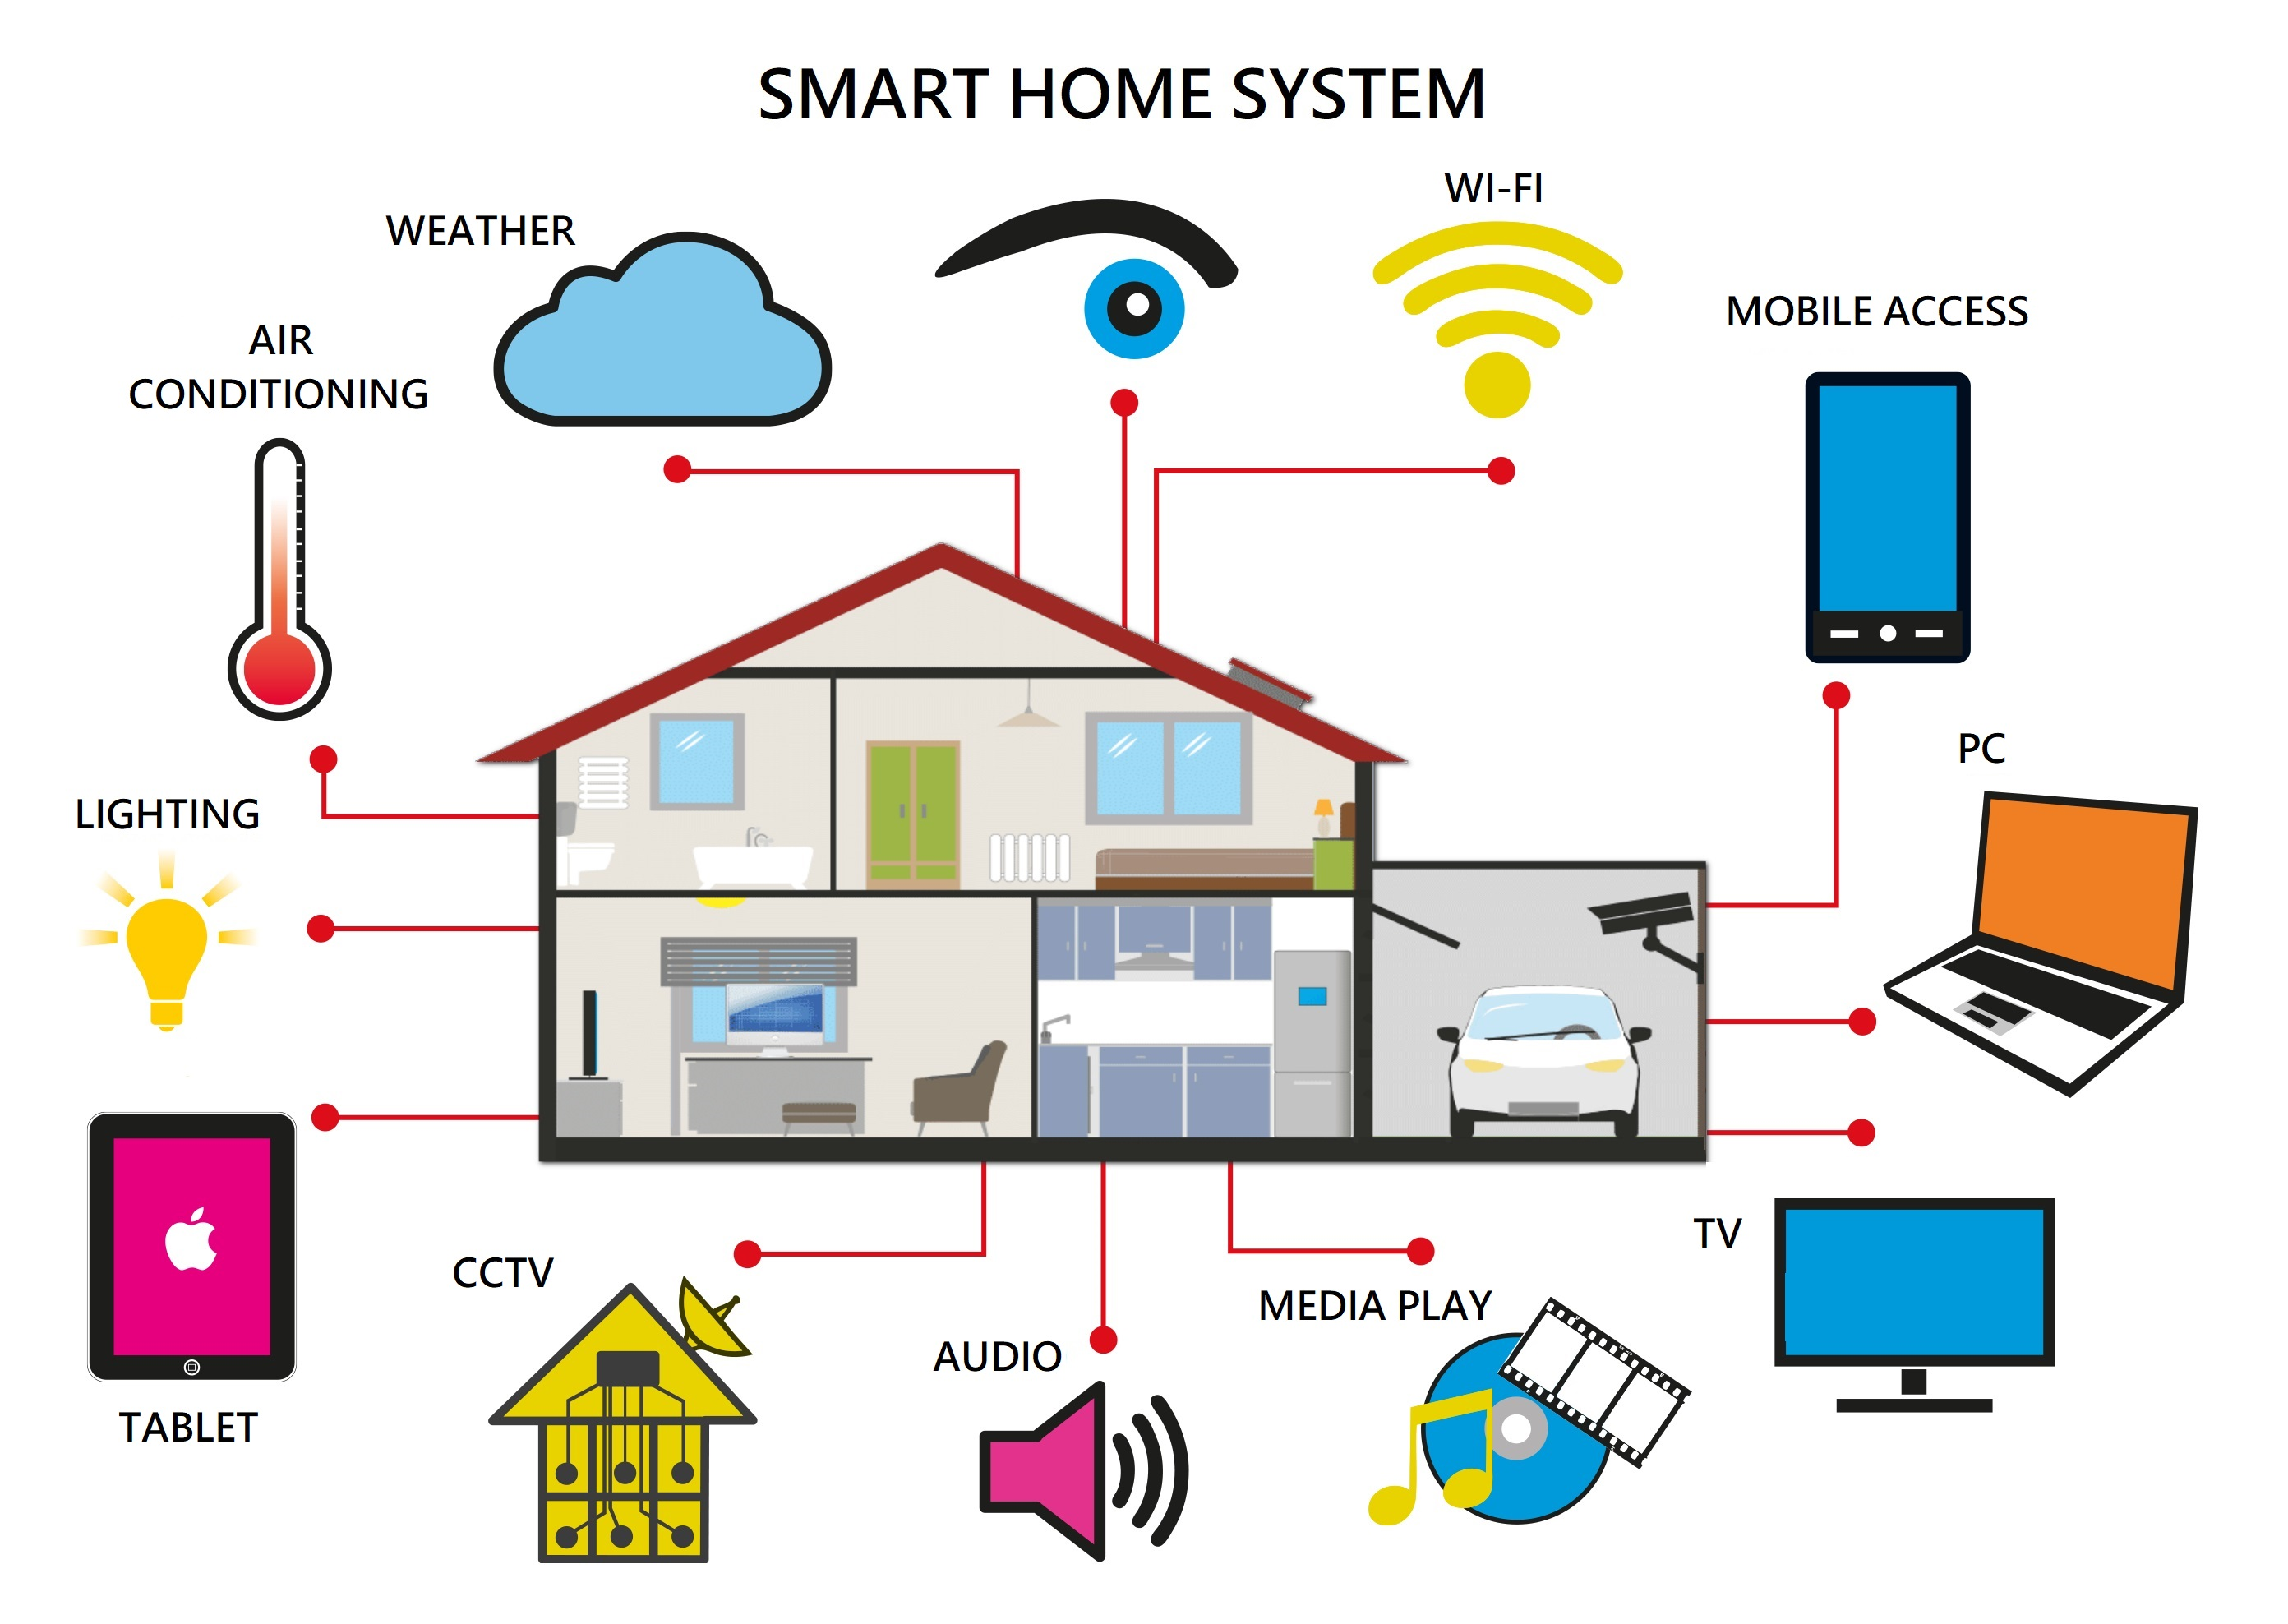
\includegraphics[width=0.9\linewidth]{Figures/Figure-01-smart-home.jpg}
\centering
\caption{Smart home system \cite{noauthor_visioforce_nodate}}
\label{fig:smarthome}
\end{figure}


\subsubsection{Temperature control devices and energy usage}

Climate control systems are required to keep the temperature and air quality within closed spaces such as houses in the desired and habitable range. The most common temperature control devices are the air conditioning units and generic fans. Fans blow air into a room which allows moisture to evaporate from an occupant’s skin thus providing that cooling effect. Air conditioners, on the other hand, pull air into a cooling and condensation mechanism, and once this cold air is radiated back into the room, a cooling effect occurs. Air conditioners are slightly more effective but use up considerably more energy to perform the same functions as a fan. To put this into context, you could have a fan running for 24 hours and it would use up as much energy as an air conditioner would use up in 15 minutes \cite{brezinski_air_nodate}. Fans are not ideal for all situations, especially when it comes to heating up a room during the cold season. However, they can replace air conditioners during the hot summers thus cutting back on electricity usage significantly. Energy conservation helps domestic consumers save money while also conserving the environment by inadvertently subverting climate change. A 3\% reduction in electricity demand would save the country about Shs.5 billion in generation capacity and Shs.1 billion in annual fuel costs \cite{noauthor_home_nodate}. According to research, buildings utilize more than 40\% of the total energy produced globally, and a majority of this energy is consumed from running air conditioning units \cite{allouhi_energy_2015}. The use of fans enables sustainable energy management thus addressing the growing difficulties of rising energy consumption and limited energy supply due to Kenya becoming more industrialized \cite{noauthor_pdf_nodate}. 
\par
As a result of rising average temperatures and extremely hot days brought on by climate change, people are anticipated to require more energy, primarily electricity for air conditioning. As a result, consumers would most likely have to spend more money on cooling due to the increased use of power \cite{reidmiller_report--brief_2018}. 


\subsection{Related Works}

% This research describes the development of an \ac{IoT} Level-4 Autonomous Smart Fan that regulates the amount of cooling based on the temperature of the room and occupants. This regulation is done automatically while the system identifies the number of people and their positions in a room and situates the best position for the fan to turn to provide a maximum cooling effect and adjusts the speed of rotation based on a predefined final temperature value.
Related research has been done in the past and some products have also been developed. For instance, a group of researchers, including Emmeline  Park and Joseph Fridlander conducted research on a smart fan that identified and tracked human movement using infrared sensors [11]. The basic premise was that fan movement and rotation would be determined by the movement of a person in a room. This research had its merits but implementation at the time was inhibited by technological deficiencies and as a result, the process stopped at the research stage.
\par
Another research team from Chittagong University of Engineering and Technology tried to replicate the smart fan incorporating infrared sensors, but the inability to distinguish between human beings and other objects curtailed their work [11]. 
\par
Vaibhav Bhatia from India and Mustafa Saad,  Hossam Abdoalgader, and Muammar Mohamed have conducted similar research on temperature-controlled fans but it stopped at the research level \cite{bhatia_room_nodate}. The research proposes using \ac{PWM} by varying the duty cycle using the room temperature and consequently varying the speed of the fan. Temperature data is acquired using a temperature sensor. The researchers focus on a ceiling fan, and while the research has merits that we can incorporate into ours, our focus rests on desk fans.
\par
Zainal, Chelvam, Seman, and Othman Designed a Low-Cost Smart Fan System using Arduino Uno. This was only for \ac{DIY} projects \cite{zainal_design_2019}. In this project, a low-cost smart fan system is designed, in which the fan's speed is determined by the room temperature. A motion sensor, temperature sensor, and a short-distance communication network made up this smart fan system. If the ambient temperature rises above a predetermined level, the fan will switch on.
\par
Woongseop Kim, Eunbi Ko, Hyebin Kim, and Eunyoung Lee, patented a Smart Fan with Face and Gesture Recognition Functions \cite{__2019}. This smart fan automatically adjusts the fan's wind direction toward the recognized user's face direction while also providing operation control functions such as fan speed and power off based on the user's gesture. It is possible to control the fan even if the user does not carry the user's equipment.
\par
Cheng Mang also patented an intelligent fan with voice control functionality \cite{_smart_2021}, while another individual, Sewoong Lee, patented a smart fan with an automatic stop function.
\par
With this it was evident that most smart fans in the market are not fully autonomous as they require user input to control the fan. While the research area is showing promise, the smart fans haven’t reached the market and users can’t enjoy their benefits.


\subsection{System}


\subsubsection{Air Flow System}

For extraction, air-conditioning, compression, and other purposes, fans are used to move gases from one location to another. They accomplish this by rotating a set of angled blades that pull air through a hole.
There are many different types of fans: impeller, axial, centrifugal, Sirocco, and so on. Each has its own set of advantages, but they all shift gases at the same pace based on the input power. Because of certain design benefits that favour one attribute over another, differences in efficiency or flow rate arise in the kind of fan.
Axial fans are a suitable design to use in this project as they have been previously used in normal fans, radiator fans and even ceiling fans. An axial fan can be depicted in figure \ref{fig:axialfandesign}.

\begin{figure}[htbp]
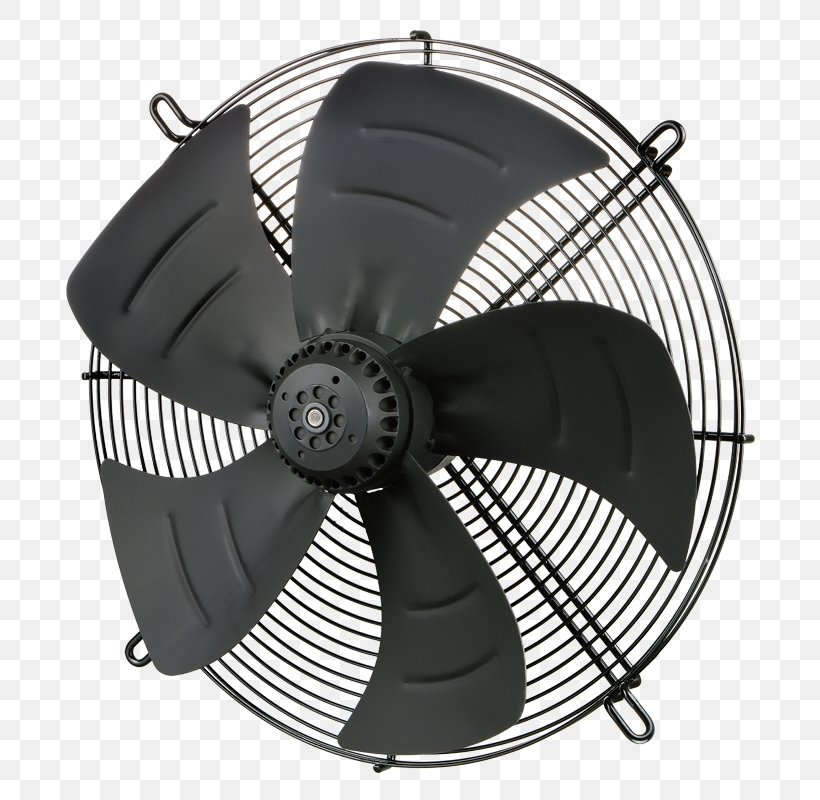
\includegraphics[scale=0.3]{Figures/Figure-02-axial-fan-design.jpg}
\centering
\caption{Axial Fan design \cite{noauthor_axial_nodate}}
\label{fig:axialfandesign}
\end{figure}


\subsubsection{Fan Blade Design}

The shape of your blades and the direction they travel will define the performance characteristics of a fan. Table \ref{table:1} shows the comparison between different fan designs based on how they are facing. The Backward facing design is the most suitable. 

\begin{table}[ht]
  \begin{center}
    \leavevmode
     \begin{tabular}{| l | c | c | c |}\hline
      Characteristic & Backward Facing & Straight & Forward Facing \\
      \hline
         Speed   & High    & Medium &   Low\\
         \hline
         Noise & Medium & Low & High\\
         \hline
         Pressure & High & Low   & Medium  \\
         \hline
         Volume Flow & Medium & Low & High \\
         \hline
         Particulates & Good & Excellent & Poor \\
         \hline
         Efficiency & 80\% & 70\% & 70\% \\
         \hline
         Construction & Heavy & Medium & Light \\
    \hline
    \end{tabular}
    \hangcaption[Different fan designs]{Different fan designs}
    \label{table:1}
  \end{center}
\end{table}


Fan calculations are based upon all the entrained air passing through the impeller with each rotation, which is normal practice for optimum blade configurations.
\par
However, too few blades, the air trailing each blade will be turbulent, reducing operational efficiency. Thus, your fan will not actually achieve the desired flow rate and pressure.
Too many blades will also reduce fan efficiency through increased skin friction and impeller mass
Table \ref{table:2} Shows how different fan blades influence the workflow of the fan

\begin{table}[ht]
  \begin{center}
    \leavevmode
     \begin{tabular}{|c | p{0.7\linewidth}|}\hline
     Number of blades & Description \\ \hline
      1 & Airflow will occur for about a third of the impeller volume, the rest of the air within the impeller will be turbulent making your fan extremely inefficient. \\
      \hline
      2 & Significantly improved airflow characteristics than one blade design but still generates significant turbulence behind each blade. Blade balancing is easier to achieve than one blade designs. \\
      \hline
      3 & Excellent for impellers with a small aspect ratio (e.g. axial fans) and much simpler to balance than 1 and 2-Blade designs. \\
      \hline
      4 & Better airflow than the 3-Blade configuration but 33\% greater skin friction. Airflow improvement more than offsets losses from skin friction. \\
      \hline
      5 & Best configuration for all medium aspect ratio impellers. \\
      \hline
      6 & Losses from increased skin friction and mass begin to exceed airflow gains. \\ \hline
    \end{tabular}
    \hangcaption[Influence of number of fan blades]{Influence of number of fan blades}
    \label{table:2}
  \end{center}
\end{table}


\subsubsection{Casing}

A fan casing may be any shape or size as long as its inlet and outlet diffusers do not impede airflow beyond that intended by the designer. Fans do not consider the manufacturing quality of the impeller casing, nor does it consider internal bends or deformations affecting the flow path.

\subsubsection{Diffuser}

The inlet area of a diffuser is the orifice nearest to the impeller. Unless the purpose of a fan is to generate suction, there is nothing to be gained by restricting inlet airflow. Therefore, the cross-sectional area of the inlet diffuser should be no less than that of the impeller blade inlet

The outlet area of a diffuser is the orifice furthest from the impeller. It is normal practice to design the diffuser outlet to minimise airflow restriction. In this case, the outlet area should be no less than that of the impeller blades.

\subsubsection{Fan Laws}

The exact relationship between speed, the diameter of the fan and efficiency is dependent on the particular design of a fan. Product testing and computational fluid dynamics are necessary to determine these design particulars. The affinity laws or fan laws express the relationships between multiple variables that determine fan performance.
\par
These laws allow a designer to determine the air flow rate from a fan by varying either the speed or diameter of the fan.
\par
Law 1. With fan diameter (D) held constant.
\par
Flow is proportional to shaft speed as shown by equation \ref{eq:1}:
\begin{equation}
\label{eq:1}
\frac{Q_1}{Q_2} = \left(\frac{N_1}{N_2}\right)
\end{equation}

Pressure is proportional to the square of shaft speed as show by equation \ref{eq:2}:
\begin{equation}
\label{eq:2}
\frac{H_1}{H_2} = \left(\frac{N_1}{N_2}\right)^2
\end{equation}

Power is proportional to the cube of shaft speed as show by equation \ref{eq:3}:
\begin{equation}
\label{eq:3}
    \frac{P_1}{P_2} = \left(\frac{N_1}{N_2}\right)^3
\end{equation}

Law 2. With shaft speed (N) held constant.
\par
Flow is proportional to the cube of fan diameter as show by equation \ref{eq:4}:
\begin{equation}
\label{eq:4}
    \frac{Q_1}{Q_2} = \left(\frac{D_1}{D_2}\right)
\end{equation}

Pressure is proportional to the square of fan diameter as show by equation \ref{eq:5}:
\begin{equation}
\label{eq:5}
    \frac{H_1}{H_2} = \left(\frac{D_1}{D_2}\right)^2
\end{equation}

Power is proportional to the fifth power of fan diameter as show by equation \ref{eq:6}:
\begin{equation}
\label{eq:6}
    \frac{P_1}{P_2} = \left(\frac{D_1}{D_2}\right)^5
\end{equation}

where:
\begin{itemize}
\item Q is the volumetric flow rate (e.g. in \ac{GPM} or L/s)
\item D is the impeller diameter (e.g. in or mm)
\item N is the shaft rotational speed (e.g. \ac{rpm})
\item H is the pressure or head developed by the fan/pump (e.g. psi or Pascal)
\item P is the shaft power (e.g. W).
\end{itemize}

\subsubsection{Specific Fan Power}
This parameter determines the amount of electric power needed to drive a fan depending on the amount of air that is circulated through the fans. It is therefore proportional to the rate of air flow as show by equation \ref{eq:7}. A designer will be able to quantify the energy efficiency of a fan by determining the specific fan power.
\begin{equation}
\label{eq:7}
    SFP = \frac{\sum P}{q_v}
\end{equation}

where:

\begin{itemize}
\item  \(\sum P\) is the electrical power used by the fan (or sum of all fans in the ventilation system) [kW]
\item  \(q_v\) is the gross amount of air circulated through the fan (or ventilation system) [m3/s]
\end{itemize}

The relationship between \ac{SFP}, fan pressure rise, and fan system efficiency as show by equation \ref{eq:8}:
\begin{equation}
\label{eq:8}
    \eta_{tot} \cdot \ac{SFP} = \Delta P_t
\end{equation}

where:

\begin{itemize}
\item  \(\eta_{tot}\) is the electrical power used by the fan (or sum of all fans in the ventilation system) [kW]
\item  \(\Delta P_t\) is the gross amount of air circulated through the fan (or ventilation system) [m3/s]
\end{itemize}

The efficiency is a function of aerodynamic losses, friction losses and other types of losses and is often in the range of 0-60\%

\subsection{Software}


\subsubsection{Communication}

To implement this design, communication between devices is constrained to wireless low energy. \ac{BLE} , \ac{UWB}, ZigBee, and
\ac{Wi-Fi} are four protocol standards for short-range wireless communications with low power consumption. They are based \ac{IEEE} standards. In general, \ac{BLE}, \ac{UWB}, and ZigBee are intended for \ac{WPAN} communication (about 10m), while \ac{Wi-Fi} is oriented to \ac{WLAN}, about 100m. However, ZigBee can also reach 100m in some applications. Lee, Su, and Shen did a comparative study of wireless protocols: \ac{BLE}, \ac{UWB}, ZigBee, and \ac{Wi-Fi} and what they found out will help make an informed decision of which technology to use \cite{lee_comparative_2007}.


\begin{table}[ht]
  \begin{center}
    \leavevmode
     \begin{tabular}{|p{3cm} | c | c | c | c |}
     \hline
        Standard & \ac{BLE} & \ac{UWB} & ZigBee & \ac{Wi-Fi}\\
      \hline
         \ac{IEEE} spec & 802.15.1 & 802.15.3a & 802.15.4 & 802.11a/b/g \\
         \hline
         Frequency band & 2.4GHz  & 3.1-10.6GHz  & 915MHz;2.4GHz & 2.4GHz;5GHz \\
         \hline
         Max Signal rate & 1 Mb/s & 110 Mb/s& 250 Kb/s &54 Mb/s \\
         \hline
         Number of RF\newline channels & 79 & 1-15 & 16 & 14(2.4GHz) \\
         \hline
         Nominal Range  & 10m & 10m &  10-100m & 100m \\
         \hline
         Nominal\newline Tx power & 0-10 dBm & -41.3 dBm/MHz & -25-0 dBm & 15 - 20 dBm \\
         \hline
         Channel\newline bandwith & 1MHz & 500MHz - 7.5GHz & 2MHz & 22MHz \\
         \hline
         Max number\newline of cell nodes & 8 & 8 & 65000 & 2007 \\
    \hline
    \end{tabular}
    \hangcaption[Comparison of the \ac{BLE}, \ac{UWB}, ZigBee and \ac{Wi-Fi} protocols.]{Comparison of the \ac{BLE}, \ac{UWB}, ZigBee and \ac{Wi-Fi} protocols.}
    \label{table:3}
  \end{center}
\end{table}


\par
\ac{BLE} is a significant protocol for \ac{IoT} applications as demonstrated by Table \ref{table:3}. It’s designed and enhanced for short-range, low bandwidth, and low latency for \ac{IoT} applications. The advantages of \ac{BLE} classic Bluetooth include lower power consumption, lower setup time, and supporting star network topology with an unlimited number of nodes \cite{samie_iot_2016}. 
\par
Even on the basis of power consumption, \ac{BLE} uses less power. This is useful in developing sensor nodes. Since it will be powered by a battery it will be wise to use the lowest energy-consuming technology.

\subsubsection{Mobile Application}

Flutter apps are written in Dart, an object-oriented programming language that resembles C.
Dart is a programming language as well as a mobile app development platform. It's used to create almost anything on the web, including servers, desktops, and, of course, mobile apps.
When Dart is used in a web application, it is converted to JavaScript so that it may run in any browser. Dart also has a Virtual Machine that allows you to run .dart files from a command-line interface. Flutter apps' Dart files are built and packed into a binary file before being uploaded to app stores. By working with Flutter for \ac{iOS} and Android at the same time, you can reach a larger audience from the start, without losing features, quality, or performance.  It is used in this product because it can help with developing the application quickly instead of using the Native Android development platform [19].

\subsubsection{Motor Control}

\ac{PWM} signal output is supported by traditional embedded systems such as Arduino. Take, for example, when the \ac{PWM} signal is always 0V (i.e., 0\% Duty Cycle), the motor is stopped from spinning. If the 5V output adds 25\% to the cycle time (i.e., 25\% Duty Cycle), the motor runs at a fourth (1/4) of its full speed. The motor spins as quickly as it can if the signal maintains a 5V output (i.e., 100\% Duty Cycle).

